%   Filename    : chapter_3.tex 
\chapter{Research Methodology}

\section{Research Activities}
\subsection{Development Framework}
The application suite is an interconnected and interdependent system, such that one feature is either dependent on or a prerequisite of another (i.e. the registration feature is required before the reporting and verification feature, the reporting and verification features are required before developing the feature that alerts and lets users to view PNP-verified cases near the user’s location, and so on).

Due to this reason, the researchers have adopted a modified version of the Feature-Driven Development (FDD) agile framework. FDD approaches software development by developing an overall model, listing all features (and how they interact), planning each feature, then focusing on designing and building one feature at a time \cite{productplan2022}. This modified version of FDD includes testing after each feature is built and integrated, and the system prototype was released only when all features have been built, integrated, and tested.

As seen in Figure \ref{fig:FDDFramework}, HanApp’s system was developed by first designing the entire model, listing all the features, planning the order by which to develop the features so that they can be integrated, and then building and integrating the features in said order.
\begin{figure}[!h]
    \centering
    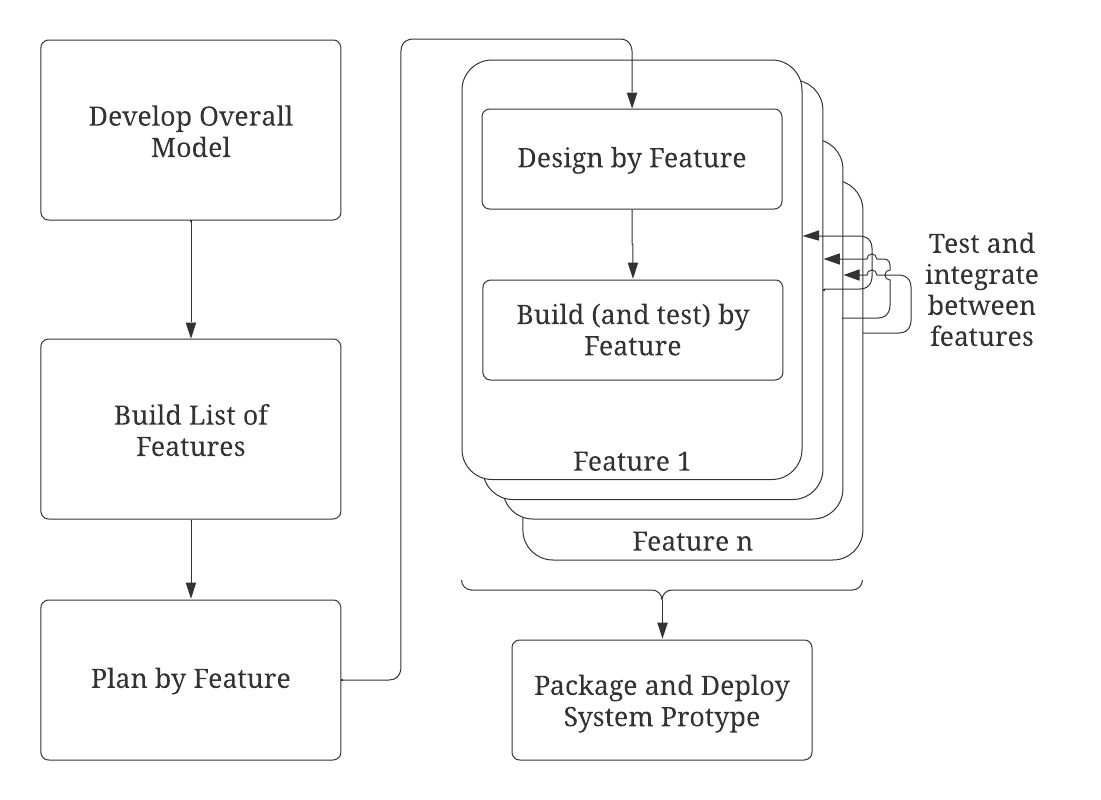
\includegraphics[width=\textwidth]{figures/Chapter3/Chapt3_DevFramework.jpeg}
    \caption{Modified Feature-Driven Development (FDD) Framework}
    \label{fig:FDDFramework}
\end{figure}

\subsection{Design, Building, Testing and Integration}

\textbf{Overall Model}

A high-level overall model or framework of what the application suite should be able to do based on general use-cases was first developed during the study’s proposal stage. It was there where the list of general features, to meet the general user requirements, were made. After which, the order of which each feature was to be designed, developed, tested, and integrated. This step ensured that each feature developed had their prerequisites met, facilitating the ease in integrating each of the application suite’s features into an overall cohesive system.

\textbf{Design and Development}

From the identified features, a rough design of how each feature would look like and how they integrate with each other was made. After which, following the FDD approach, each feature was designed and consequently developed, with the frontend (UI/UX) and backend (functions, data handling) codes of each feature being developed simultaneously.

\textbf{Testing and Integration}

During and after the development of each feature, the feature is user-tested in order to ensure that the features work as intended and any bugs are immediately fixed. For features that rely on previous features to work (i.e. user account creation must work before user login), extensive user testing was done to confirm that the integration between each feature worked as intended. 

Due to both time and technical constraints, testing was done solely by user testing rather than written and automated tests. Once the current feature and its prerequisite features have been tested, the development of the next feature would commence.

\textbf{Implementation}

The final prototype is the fully functional application suite (including all the user interfaces) that meets the users’ requirements and passes all the tests during development.

\textbf{System Prototype}

The final product of the study, the HanApp main user app and the PNP app, is made available to the intended users. In this phase, routine maintenance and regular performance monitoring, particularly in the backend (traffic, database health, storage usage, API usage), is required to keep the application running smoothly. Post-release support would also include bug reporting and fixes, as well as backend and frontend optimizations to enhance the application’s efficiency and availability.

\section{Development Tools}
\subsection{Software}

\subsubsection{Github}
GitHub is a web-based tool that utilizes Git, an open source version control that enables several users to make distinct modifications to applications or software simultaneously \cite{digitalGovGitHub}. GitHub is currently being used by over 94 million software developers, 4 million plus organizations, and has created over 330 million repositories for varied software \cite{github}. 

Github was utilized in the project for storing the source code of the application suite and for the source version control during development, as well as for the repository for the LaTeX files for the study itself.

\subsubsection{Visual Studio Code}
Visual Studio Code (VS Code) is a compact yet capable source code editor for macOS, Windows, and Linux that runs on your desktop. It supports multiple programming and scripting languages like JavaScript, TypeScript, and Node.js, as well as a robust ecosystem of extensions for additional languages and runtimes (including C++, C\#, Java, Python, PHP, Go, and.NET) \cite{microsoft_2021}.

Visual Studio Code and Android Studio were used simultaneously as the primary source code editor, with Android Studio's Android Emulator being used to run the debug builds of the application suite.  

\subsubsection{Android Studio}
Android Studio is the official Integrated Development Environment (IDE) for developing Android mobile apps. It is based on the IntelliJ IDEA development tools and code editor. When compared to other IDEs, Android Studio is considered hefty; however, this is expected considering that it incorporates various integrations and add-ons like a flexible Gradle-based build system, built-in emulators, code templates, extensive testing tools, and many others to guarantee that development is as interactive and fluid as possible \cite{androidStudio}.

Android Studio comes with an Android Emulator which was the primary tool used for running and testing the application interfaces, as well as in debugging.

\subsubsection{Flutter}
Flutter is a Google open-source framework used for creating attractive, locally built, multi-platform apps out of a single codebase. For rapid efficiency and performance on any device, Flutter code compiles to ARM or Intel machine code, as well as JavaScript. Dart, a programming language designed for speedy programs on any platform, powers it \cite{flutter}. As the developers have aimed to deploy the proposed application on both the mobile (Android) platform for the main users, and on the Web (desktop)  platform for the side of PNP, Flutter is an outstanding choice out of all the available frameworks and languages.

Flutter (and the Dart programming language) was utilized in the development of all HanApp's interfaces. Flutter packages were also imported for ease of feature development.

\subsubsection{Google Firebase}
As Firebase has a variety of products and services that it provides, such as Firebase Auth, which is a service that can authenticate users using only client-side code, Real-time Database, a NoSQL database service, and Firebase Storage, which is a file transfer service \cite{khawas2018application}, Firebase remains to be the most optimal choice for a serverless mobile application that may require the said services, such as with the proposed application.

Google Firebase is the sole and primary backend of the application suite. User authentication, database and data storage, and usage monitoring were all done under Firebase. Since Firebase is a serverless framework, utilizing Firebase as the application suite's backend allowed for development and testing without the use of a dedicated server infrastructure. 

\subsubsection{Google Maps}
Google Maps, one of the world’s most influential applications \cite{mehta2019google}, provides multiple location services needed in the proposed application. This includes the pinging of the location of the user of the companion app, or perhaps even the pinpointing and updating of the location where a verified missing person was last seen.

\subsection{Hardware}
\subsubsection{Android Phone}
An Android phone is a type of smartphone that is operating using the operating system developed by Google, Android. Apart from the Android Studio's Android Emulator,  physical Android phones were utilized to test the debug and release builds of the application suite's main user mobile interface.

\subsubsection{Laptop}
The application was developed on laptop computers with the minimum specifications of an 8th generation Intel Core i3 CPU, and 8GB of RAM.

\subsection{Packages and Application Programming Interfaces (APIs)}

\subsubsection{Packages}
Software packages are a group of software programs that can be downloaded as a bundle of related products and used in the development of software.  They provide functionalities that are editable or customizable, in order to adjust to the specific requirements of organizations or developers that uses them \cite{jadhav2009evaluating}.

Packages in Flutter can be reviewed and downloaded from pub.dev, the official package archive for Flutter and Dart applications, which is also supported by Google \cite{pubdev}. Throughout the development of the applications, multiple verified packages from pub.dev have been used and are now essential to the functionality of the applications.

\paragraph{Firebase Packages.} Multiple Firebase packages from pub.dev have been utilized in the development of the application to better integrate the serverless backend service (Firebase) onto the applications' interface and services. These packages are firebase\_core, the overall prerequisite and helper package for all Firebase services in the Flutter application \cite{firebaseCore}, firebase\_auth, the package utilized in order to facilitate the registration, verification, log-in, and authentication persistence of users of the applications \cite{firebaseAuth}, and firebase\_storage and firebase\_database for the cloud storage needed by the images utilized by the applications, and the real-time database (RTDB) used to save multiple data needed by the applications \cite{firebaseAuth, firebaseStorage}.

\paragraph{Location Packages.} Packages were also needed in order to better facilitate and integrate maps and location services on the applications. These packages are google\_maps\_flutter, google\_maps\_flutter\_web, and location. The aforementioned google maps packages are used on the mobile application and the web applications respectively, for they are needed in order to display and better blend the user experience for using google maps services on the applications' targeted platforms. Location package, on the other hand, was used in order to ask for user permission before the application requests their current device's location.

\paragraph{Data Persistence Package.} Data persistence between views and states of the application is crucial in order to properly pass on volatile data from one page or interface, onto another within the application. For this purpose, the package shared\_preferences was used. This package allowed the developers to save data within the application itself or from the databases into a key-value pair in the platform-specific persistent storage for simple data like Strings and Boolean values, among other types \cite{sharedPreferences}.

\subsubsection{Application Programming Interfaces (APIs)}

\paragraph{Geocoding API.} The Geocoding API converts addresses directly into geographic coordinates, which may then be used to set markers on a map or position the map  \cite{geocoding}.

\paragraph{Maps SDK for Android API.} Maps SDK for Android is an API from the Google Cloud suite that adds maps functionality to Android apps and even on some embedded systems like Wear OS. This API enables Android-based hardware to use Google maps data, maps display, and maps gestures and responses. Additionally, it also provides some needed customizability on the maps interface by drawing polygons, lines, shortest paths, and customizable markers \cite{androidSDK}. 

\paragraph{Maps JavaScript API.} Maps JavaScript API is another API from the Google Cloud suite that enables maps functionality, customizability, and imagery for display on the web. The API features four map types, namely; roadmap, hybrid, terrain, and satellite \cite{javascriptSDK}.

\section{Application Requirements}

\subsection{Backend Requirements}

Listed below is the overall structure of all connections and relationships among all data, interfaces, users, and the serverless service. 

\subsubsection{Serverless Architecture}

\begin{figure}[!h]
    \centering
    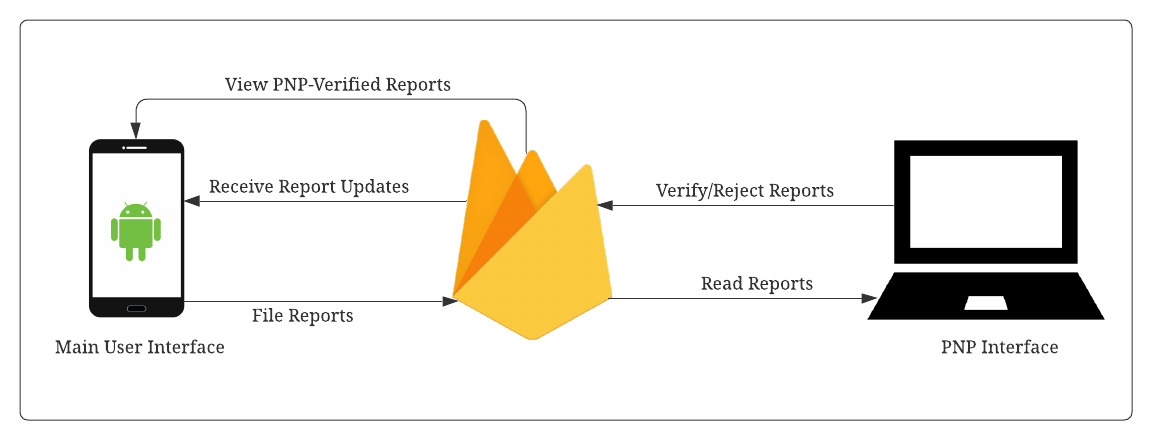
\includegraphics[width=\textwidth]{figures/Chapter3/Chapt3_ServerlessArchitecture.jpeg}
    \caption{Client-Serverless Architecture with Firebase}
    \label{fig:ServerlessFirebase}
\end{figure}

The overall serverless architecture of the application suite and its system is portrayed in the diagram above. Firebase, as the serverless service being utilized, serves as the storage medium for all data being utilized in all of HanApp’s interfaces. 

\subsubsection{Realtime Database structure for Main User and PNP profiles}

Each profile type will be a node just under the root node as child nodes, namely, Main Users, and PNP Admins. 

\subsubsection{Realtime Database structure for sent reports}
As Firebase’s real-time database is structured as a tree, sent reports will be listed as child nodes of the user who sent them. This way, it will be easier to know who has filed what, and only the user who has filed an unverified report can directly see it. Once the PNP Admin interface has verified it, then that report will be displayed publicly.

\subsubsection{Images and other media storage}
The real-time database only functions on non-media data like text, integers, and location data; therefore, images used within the application interfaces (user image, missing person image) will be stored in Firebase’s cloud storage. 

\subsection{User Interface Requirements}
\subsubsection{User (or Main) Interface}

\begin{figure}[!h]
    \centering
    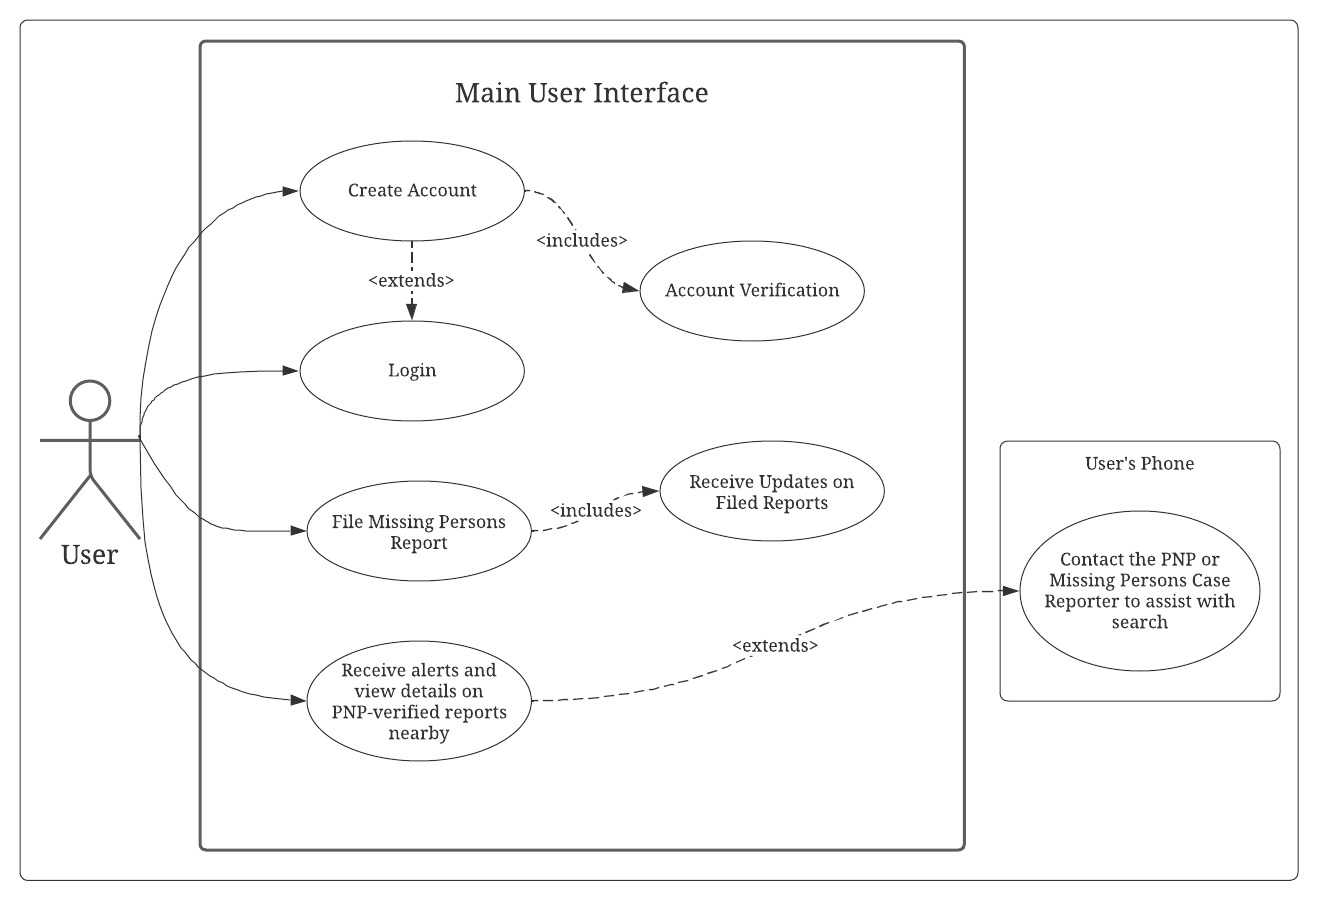
\includegraphics[width=\textwidth]{figures/Chapter3/Chapt3_UseCase_Main.jpeg}
    \caption{Use-Case Diagram for User (Main User Interface)}
    \label{fig:UseCaseMain}
\end{figure}
The User use-case diagram in Figure \ref{fig:UseCaseMain} illustrates all the possible tasks that a normal user could do within the main user application. User account creation will be done within the application itself, through Firebase Auth’s authentication service using a registered email address and password. After the user has registered and confirmed their email address, their account will be created. The main feature within the application is with the reporting of missing persons. This is done through the application by filling out a form with the details required for the missing persons report, which would then be filed towards the most logically sound police-station. Users can also receive notifications with regards to the descriptions and features of any missing persons report that have been verified by the PNP.

\subsubsection{PNP Admin App Interface}

The PNP and PNP Admin interface use-case diagram is shown in Figure \ref{fig:UseCasePNP}. The PNP admin accounts are created in a different manner compared to the previously stated accounts. First, PNP admin accounts cannot be created through the PNP admin interface (e.g., a ``Register" option) in order to control and limit the number of admin users within a police station to only one, who can only handle missing persons reports within their vicinity. 

Local police stations can request PNP admin accounts from the developers in order for it to be recognized as an ``admin" account rather than any other user account . Once a PNP admin has logged in to the PNP admin interface, he or she, as an official, can then browse and either verify or reject missing person reports filed within their jurisdiction.
\begin{figure}[!h]
    \centering
    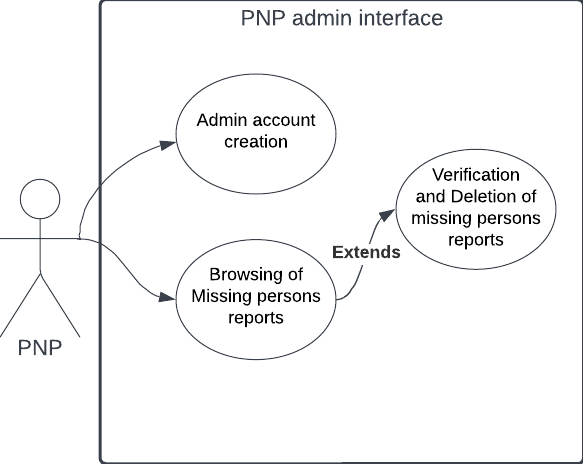
\includegraphics[scale=0.5]{figures/Chapter3/Chapt3_UseCase_PNP.png}
    \caption{Use-Case Diagram for PNP (PNP Admin Interface)}
    \label{fig:UseCasePNP}
\end{figure}


\subsection{Functional Requirements}

The following are the user requirements, for both the main users and PNP users, identified during the design phase of the application suite's development in order to meet the study's objectives. 

\subsubsection{User Registration}
Main application users should be able to launch their respective application interfaces and register through the log-in and registration page in-app. Once verified and registered, users can then utilize and log in into the application. 

\subsubsection{PNP Admin Account Creation}

For security reasons, creation of PNP Admin accounts will be highly regulated. As such, for the initial release build of the application suite, the PNP accounts are created upon the PNP's request to the developers to create their admin account.

As proof of concept and for testing purposes, the PNP Admin test accounts will be hard-coded by the developers to simulate the process of PNP requesting for an account. 


\subsubsection{Reporting and Receiving Updates}
General users should be able to fill out and send the MP case report form via the main app interface to the PNP station where the reported person went missing has the closest vicinity to, and receive updates via the main app with regards to the status of the report.

With regards to reporting, it is of utmost importance that the report form pages of the main user interface should be intuitive, and be able to condense and simplify the forms required in the PNP's guidelines on reporting missing persons cases.

\begin{figure}[!h]
    \centering
    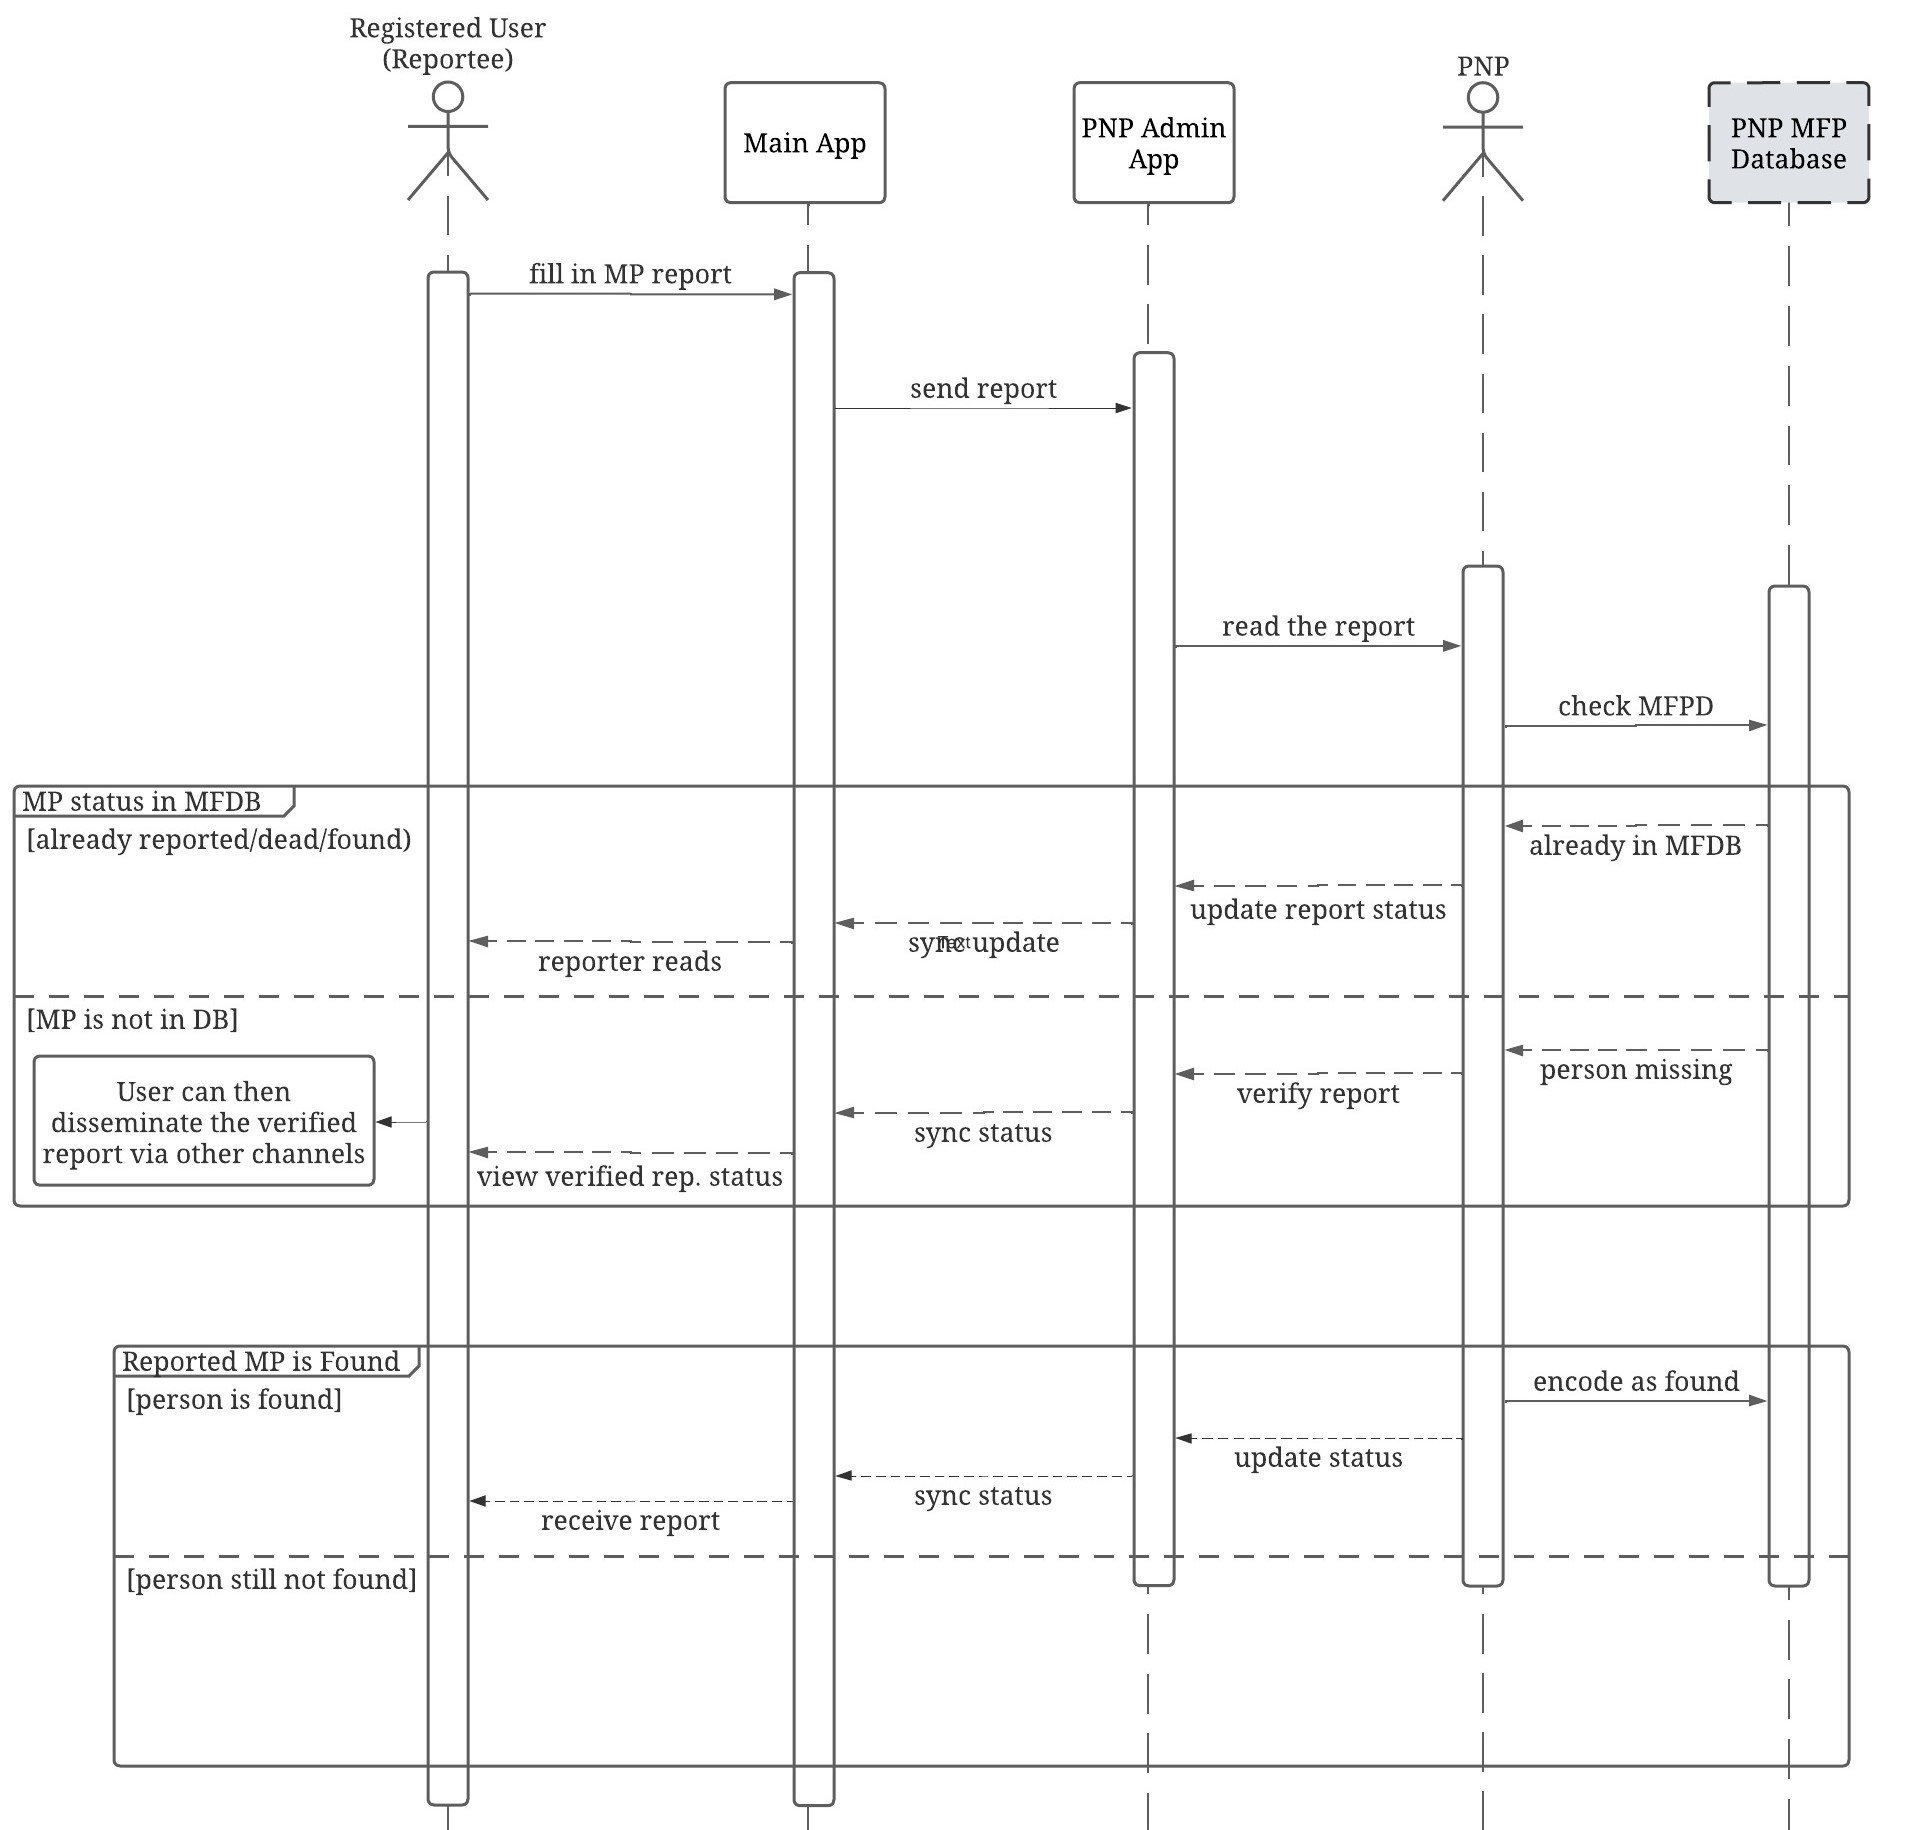
\includegraphics{figures/Chapter3/Chapt3_seqDiag_report.jpeg}
    \caption{Sequence Diagram for Reporting, Updating, and Verification of MP cases}
    \label{fig:seqDiaReport}
\end{figure}
As seen in Figure \ref{fig:seqDiaReport} sequence diagram, reporting and receiving updates is very straightforward: the user (reportee) needs to fill out the MP report form, it’s received by the PNP through their PNP Admin App interface, and if the person is indeed missing (and not yet reported, or registered as already found or dead in the PNP's own Missing and Found Person Database (MFPD)), then the PNP can verify the report. If any updates are made, such as if the MP is found, it will be reflected in the user’s app soon after.

\begin{figure}[!h]
    \centering
    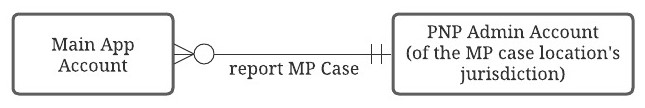
\includegraphics[width=\textwidth]{figures/Chapter3/Chapt3_ERDiag_reporteePNP.jpeg}
    \caption{Entity Relationship Diagram of Main App Account Reporting to PNP Admin Account}
    \label{fig:ERDReportee}
\end{figure}
It’s also an important requirement that any reports made by users (reportee) are sent to the PNP Admin Account of the A/MP's last known location’s nearest PNP station, as mentioned prior. As seen in Figure \ref{fig:seqDiaReport} , many users should be able to submit MP case reports of a specific location to the PNP through the application, but they will only be routed to the PNP Admin Account registered for said location.

\subsubsection{Receive, Update, and Verify Reports}

The PNP Admin should be able to receive reports from users through the PNP Admin app. PNP Admin should also be able to put updates on the report (i.e. MP case already reported, MP reported is already found, etc.), and also verify the report to state that the MP is categorized as missing. This can also be seen in the sequence diagram in Figure \ref{fig:seqDiaReport}. 

\subsubsection{Accessing PNP-Verified Reports and receiving Location-based notification for PNP-verified MP cases}

Users in a certain radius of the PNP-verified MP case  should receive notifications about an MP case in their area. Users can tap on the marker where the MP was last seen to view the concise details of the MP in the report. As seen in Figure \ref{fig:diagramLocation}, all users should be able to view all PNP-verified reports, including those outside their radius, but will only receive notifications for cases within the user's radius.

\begin{figure}[!h]
    \centering
    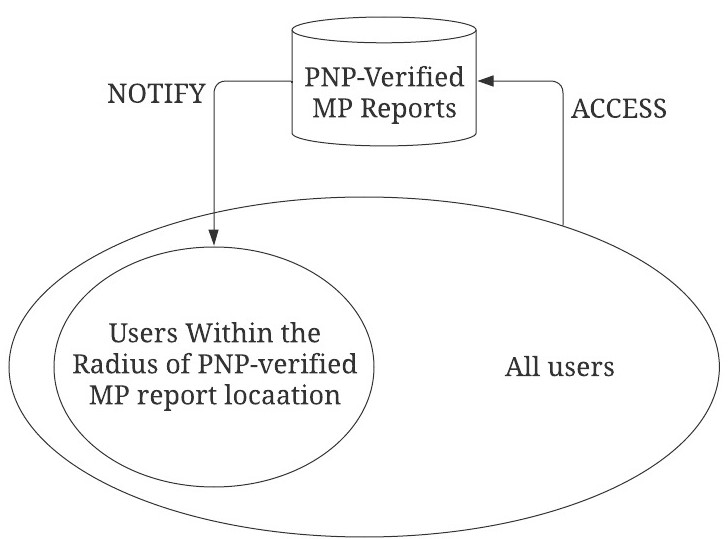
\includegraphics[scale = 1.50]{figures/Chapter3/Chapt3_Diag_locationBasedNotif.jpeg}
    \caption{Diagram for PNP-Verified Reports Access and Notification System}
    \label{fig:diagramLocation}
\end{figure}